% TODO: reorganizar este apêndice para fazer mais sentido

\begin{apendicesenv}
\partapendices

\chapter{Descrição matemática do modelo de micelas gigantes}

\section{Introdução e motivação}

% TODO: colocar as referências.
Esta seção mostrará as equações utilizadas para descrever o modelo de espalhamento de micelas gigantes. As equação foram baseadas numa série de artigos de X, Y, Z. Aqui, esses artigos serão agrupados, de modo a facilitar o entendimento do modelo.

Porém, essa descrição matemática é de menor aplicabilidade, pois é necessário transcrever as equações em código que consiga realizar ajustes. Essa tarefa não é trivial, especialmente para não especialistas. Logo, será disponibilizado, na seção X, uma transcrição dessas equações, na linguagem Python.

% TODO: colocar a seção onde o modelo foi utilizado
% TODO: colocar a seção onde a descrição de Python foi escrita
% TODO: reescrever essas equações, colocando os termos qe são texto em \text e o resto normal

\section{Resumo do modelo}

O modelo descreve cadeias alongadas caroço-casca (\emph{core-shell}) de Kratky-Porod, considerando volume excluído, com interações intercadeias modeladas pelo modelo PRISM (\emph{Polymer Reference Interaction Site Model}). No total, a equação de intensidade de espalhamento $I$ em função do vetor de espalhamento \q ($I(q)$, Eq. \ref{eqn:AP_saxs_MG_superficial}) possui 13 parâmetros, descritos na tabela \ref{tab_ap:simbolos}.

\begin{equation}
I = f(q, scale, d_{head}, r_{core}, \rho_{rel}, \sigma, back, L, k_L, \varepsilon, D_{CQ}, \nu_{RPA}, SC_{pow}, exp_{pow})
\label{eqn:AP_saxs_MG_superficial}
\end{equation}
% TODO: colocar refs às equações que definem alguns desses termos
\begin{table}
    \IBGEtab%
    {\caption{Símbolos e parâmetros utilizados no modelo, e seus significados}
     \label{tab_ap:simbolos} }%
    {\begin{tabular}{r p{8cm}}
    	\toprule
     Símbolo 			& Descrição        						\\
     \midrule
     $I$					& Intensidade de RX espalhado			\\
     \q					& Vetor de espalhamento					\\
     \midrule
     $scale$				& Fator de escala						\\
     $d_{head}$			& Espessura do \emph{shell}				\\
     $r_{core}$			& Raio do \emph{core}					\\
     $\rho_{rel}$		& Diferença de densidade eletrônica entre \emph{core} e \emph{shell} \\
     $\sigma$			& Fator de \emph{smearing}, o quão definido é o limite entre regiões \\
     $back$				& Constante referente ao \emph{background} \\
     $L$					& Comprimento de contorno das cadeias 	\\
     $k_L$				& Comprimento de \emph{Kuhn} das cadeias, igual ao dobro do comprimento de correlação \\ % TODO: Achar o que é esse comprimento exatamente
     $\varepsilon$			& Excentricidade radial das micelas		\\
     $D_{CQ}$			& Distância de correlação das micelas 	\\
     $\nu_{RPA}$			& Fator de concentração					\\
     \midrule
     $SC_{pow}$			& Fator de escala (pre-exponencial) da exponencial em baixo q\\
     $exp_{pow}$			& Fator exponencial, relativo à inclinação na escala log\\
     \bottomrule
    \end{tabular}}%
    {}%
\end{table}

A equação geral do modelo, e a descrição de seus fatores, estão descritos na Eq.\ref{eqn:AP_saxs_MG_geral} e na Tab. \ref{tab_ap:fatores_geral}.

\begin{equation}
I = \frac{scale\left(F_{KPchain_{ExV}}F_{rod_{CS}}\right)}{1 + \nu_{RPA} F_{sphere}\left( D_{CQ}\right) F_{KPchain_{ExV}}} + back + scale_{pow}^{-exp_{pow}}
\label{eqn:AP_saxs_MG_geral}
\end{equation}

\begin{table}
    \IBGEtab%
    {\caption{Parâmetros da equação \ref{eqn:AP_saxs_MG_geral}}
     \label{tab_ap:fatores_geral} }%
    {\begin{tabular}{r p{8cm}}
    \toprule
    Termo 			& Descrição        						\\
    \midrule
    $F_{KPchain_{ExV}}$  & Fator forma de cadeias de Kratky-Porod com volume excluído \\
    $F_{rod_{CS}}$		 & Fator forma da seção transversão de um bastão	\\
    $F_{sphere}(D_{CQ})$ & Fator forma de uma esfera, cujo raio é a distância de correlação \\
    \bottomrule%
    \end{tabular}}
    {}%
\end{table}


Já o modelo do PRISM é descrito pela Eq. \ref{eqn:AP_saxs_PRISM}. Note a similaridade com a Eq \ref{eqn:AP_saxs_MG_geral}.

\begin{equation}
I_{PRISM}= \frac{\varphi V_{mic}F_{wc}(q)F_{cs}(q)}{1 + \nu F_{rod}(qL_{c(q)})F_{wc}(q)}
\label{eqn:AP_saxs_PRISM}
\end{equation}

\begin{table}
    \IBGEtab{%
      	\caption{Termos da equação \ref{eqn:AP_saxs_PRISM}}
    \label{tab_ap:PRISM_geral}}%
    {%
     \begin{tabular}{r p{8cm}}
     \toprule
     Termo 			& Descrição        						\\
     \midrule
     $\varphi$		& Fração volumétrica \\ % TODO: checar
     $V_{mic}$		& Volume da micela   \\
     $F_{wc}$		& Fator forma de uma \emph{wormlike chain} \\
     $F_{cs}$		& Fator forma de uma seção transversal de cilindro \\ % TODO: checar se é cilindro
     $F_{rod}$		& Fator forma de um bastão infinitamente longo \\
     $L_{c(q)}$		& $=6\xi$, comprimento característico \\
     $\xi$			& Comprimento de correlação da função $c(q) \approx F_{rod}$ \\
     \bottomrule
     \end{tabular}}%
     {}%
\end{table}


A partir disso, podemos começar a adentrar nos termos.

\section{Descrição detalhada do modelo}

O modelo será dividido em duas partes, uma referente à cadeia micelar, $F_{wc}$ e outra referente à seção transversal da cadeia, $F_{cs}$.

\subsection{Fator forma das cadeias \emph{wormlike}, $F_{wc}$}
\label{sec:equacoes_Fwc}

\begin{equation}
F_{wc} = \left[\left(1 - \chi\right)F_{chain_{ExV}} + \chi F_{rod}\right]\Gamma
\label{eqn:AP_Fwc}
\end{equation}

% TODO: colocar a equação do \Gamma
A equação \ref{eqn:AP_Fwc} pode ser simplificada dependendo da faixa de \q. A região de \q intermediária precisa ser descrita pelo termo $\chi$ (Eq. \ref{eqn:AP_chi}) e corrigida por $\Gamma$. Esses parâmetros são obtidos por simulações de Monte Carlo.

\begin{equation}
	F_{\text{wc}} \approx 
		\begin{cases}
			F_{\text{chain}_{\text{ExV}}}		& \text{q baixo}  \\
			F_{\text{rod}}						& \text{q alto}
		\end{cases}
	\label{eqn:AP_Fwc_dois_casos}
\end{equation}

%	\begin{longtable}[c]{r p{12cm}}
%		\toprule
%		Termo 			& Descrição        						\\
%		\midrule
%		$\chi$			& Região de \emph{crossover} \\
%		$\Gamma$		& Correção da região de crossover. \\
%		\bottomrule
%		\caption{Termos da equação \ref{eqn:AP_Fwc}}
%		\label{tab_ap:Fwc} 
%	\end{longtable}

\subsubsection{Fator de correção $\chi$}
O termo $\chi$ é descrito pela equação \ref{eqn:AP_chi}, que por sua vez é dependente da equação \ref{eqn:AP_xi}.

\begin{equation}
\chi = \exp{\xi^{-5}}
\label{eqn:AP_chi}
\end{equation}

% todo: achar o significado do termo b
\begin{equation}
\xi = q k_L\left(\frac{\pi b}{1,103L}\right)^{3/2}\left(\frac{\left<R_g^2\right>}{k_L^2}\right)^{1,282}
\label{eqn:AP_xi}
\end{equation}

\noindent onde $\left<R_g^2\right>$ é a média do \emph{ensemble} do quadrado do raio de giro das cadeias, no modelo.

\subsubsection{Fator forma de cadeias com volume excluído, $F_{chain_{ExV}}$}
\label{sec:F_chain_ExV_equacoes}
O termo $F_{chain_{ExV}}$ possui a seguinte forma (Eq. \ref{eqn:AP_FchainExV})

% TODO: verificar se o \nu aqui é o \nu_RPA
\begin{multline}
F_{chain_{ExV}} = w(qR_g)F_{Debye}(q,L,k_L) + \left[1 - w(q R_g)\right] \\ \left[C_1(q R_g)^{\frac{1}{\nu}} + C_2(q R_g)^{-\frac{2}{\nu}} + 
C_3(q R_g)^{-\frac{3}{\nu}}\right]
\label{eqn:AP_FchainExV}
\end{multline}
% todo: colocar o valor de \nu, que está na Eq. S_EXV_APP
% todo: incluir aqui uma tabela com os termos e as equações

O termo $F_{Debye}$, por sua vez, é dado pela Eq. \ref{eqn:AP_fdebye}.
\begin{equation}
F_{Debye} = 2 \left(\frac{e^{-u} + u - 1}{u^2}\right)
\label{eqn:AP_fdebye}
\end{equation}

\noindent onde $u = R_g^2q^2$. $R_g$ é a raiz quadrada do raio de giro médio ao quadrado, $R_g = \left<R_g^2\right>^{1/2}$, considerando o volume excluído. Por sua vez, esse valor é dado pela Eq. \ref{eqn:AP_Rg2}

% todo: Achar o que significam os termos faltantes aqui.
\begin{equation}
\left<R_g^2\right> = \alpha \left(\frac{L}{k_L}\right)^2\left<R_g^2\right>_0
\label{eqn:AP_Rg2}
\end{equation}

O termo $w$ é uma equação empírica, da forma: (Eq \ref{eqn:AP_w})

\begin{equation}
w(x) = \frac{\left[1 + \frac{\tanh(x-C_4)}{C_5}\right]}{2}
\label{eqn:AP_w}
\end{equation}

As constantes $C_1$, $C_2$, $C_3$, $C_4$ e $C_5$ foram obtidas a partir de um ajuste, e estão na tabela \ref{tab_ap:C1C5}, assim como o valor de $\nu$.
\begin{table}
    \IBGEtab%
    {\caption{Constantes}
    \label{tab_ap:C1C5} }%
    {\begin{tabular}{r p{2cm}}
      \toprule
      Constante 	& Valor \\
      \midrule
      $C_1$			&  1,220	\\
      $C_2$			&  0,4288	\\
      $C_3$			&  -1,651	\\
      $C_4$			&  1,523	\\
      $C_5$			&  0,1477 	\\	
      $\nu$			&  0,585	\\					
      \bottomrule
    \end{tabular}}% todo: encontrar de onde vem o \nu
    {}%
\end{table}


\subsubsection{Fator de correção $\Gamma$}

O fator de correção $\Gamma$ (Eq. \ref{eqn:AP_Gamma}) é dependente de dois conjuntos de constantes, $A$ (Eq. \ref{eqn:AP_Ai}) e B (Eq. \ref{eqn:AP_Bi}) determinadas empiricamente (Tab \ref{tab_ap:AiBi}).

\begin{equation}
\Gamma\left( q,L,k_{L} \right) = 1 + \left( 1 - \chi \right)\sum_{i = 2}^{5}{A_{i}\xi^{i}} + \chi\sum_{i = 0}^{2}{B_{i}\xi^{- i}}
\label{eqn:AP_Gamma}
\end{equation}

\begin{equation}
A_{i} = \sum_{j = 0}^{2}{a_{1}\left( i,j \right)\left( \frac{L}{k_{L}} \right)^{- j}\exp\left( - \frac{10k_{L}}{L} \right)} + \sum_{j = 1}^{2}{a_{2}\left( i,j \right)\left( \frac{L}{k_{L}} \right)^{j}\exp\left( - \frac{2L}{k_{L}} \right)}
\label{eqn:AP_Ai}
\end{equation}

\begin{equation}
B_{i} = \sum_{j = 0}^{2}{b_{1}\left( i,j \right)\left( \frac{L}{k_{L}} \right)^{- j}\ } + \sum_{j = 1}^{2}{b_{2}\left( i,j \right)\left( \frac{L}{k_{L}} \right)^{j}\exp\left( - \frac{2L}{k_{L}} \right)}
\label{eqn:AP_Bi}
\end{equation}

\begin{table}[h]
    \IBGEtab%
    {\caption{Constantes utilizadas para o cálculo de $\Gamma$}
    \label{tab_ap:AiBi}}%
    {\begin{tabular}{r l | r l | r l | r l}
    \toprule
    $a_1$(2,0) & --0.1222 & $a_2$(2,1) & 0.1212 & $b_1$(0,0) &
    --0.0699 & $b_2$(0,1) & --0.5171\\
    $a_1$(3,0) & 0.3051 & $a_2$(3,1) & --0.4169 & $b_1$(1,0) & --0.09
    & $b_2$(1,1) & --0.2028\\
    $a_1$(4,0) & --0.0711 & $a_2$(4,1) & 0.1988 & $b_1$(2,0) &
    0.2677 & $b_2$(2,1) & --0.3112\\
    $a_1$(5,0) & 0.0584 & $a_2$(5,1) & 0.3435 & $b_1$(0,1) & 0.1342
    & $b_2$(0,2) & 0.6950\\
    $a_1$(2,1) & 1.761 & $a_2$(2,2) & 0.0170 & $b_1$(1,1) & 0.0138 &
    $b_2$(1,2) & --0.3238\\
    $a_1$(3,1) & 2.252 & $a_2$(3,2) & --0.4731 & $b_1$(2,1) & 0.1898
    & $b_2$(2,2) & --0.5403\\
    $a_1$(4,1) & --1.291 & $a_2$(4,2) & 0.1869 & $b_1$(0,2) & --0.2020
    & &\\
    $a_1$(5,1) & 0.6994 & $a_2$(5,2) & 0.3350 & $b_1$(1,2) & --0.0114
    & &\\
    $a_1$(2,2) & --26.04 & & & $b_1$(2,2) & 0.0123 & &\\
    $a_1$(3,2) & 20.00 & & & & & &\\
    $a_1$(4,2) & 4.382 & & & & & &\\
    $a_1$(5,2) & 1.594 & & & & & &\\
    \bottomrule
   \end{tabular} }%
    {}%
\end{table}

\subsubsection{Fator forma de um cilindro $F_{rod}$}

O fator forma de um cilindro segue a equação \ref{eqn:AP_Frod}.

\begin{equation}
F_{rod}(q, L) = \frac{2Si(qL)}{qL} - \frac{4\sin^2\frac{qL}{2}}{q^2L^2}
\label{eqn:AP_Frod}
\end{equation}

\noindent onde $Si$ é a função-integral de seno (Eq. \ref{eqn:AP_Si})

\begin{equation}
Si(x) = \int_0^x \frac{\sin t}{t}dt
\label{eqn:AP_Si}
\end{equation}

% TODO: verificar se F_CS é de fator da seção de um cilindro. CS é cross section mesmo.
\subsection{Fator forma da seção transversal de um cilindro $F_{cs}$}

O fator forma da seção transversal de um cilindro é descrito pela equação \ref{eqn:AP_Fcs}. Seus parâmetros se encontram na tabela \ref{tab_ap:Fcs}

\begin{equation}
F_{\text{cs}} = \frac{2}{\pi}\int_{0}^{\frac{\pi}{2}}%
%
\left[ \left(\rho_{S} - \rho_{w} \right) \frac{2J_1 \left( qR_{S}\left( \varepsilon,\theta \right) \right)}{qR_{S}\left( \varepsilon,\theta \right)} % 
%
+  %
%
\frac{\pi\varepsilon R_C^2}{\pi\varepsilon R_S^2}\left( \rho_c - \rho_s \right)	%
%
\frac{2J_1\left( qR_{C}\left( \varepsilon,\theta \right) \right)}{qR_{C}\left( \varepsilon,\theta \right)}\  \right]^2 d\theta
\label{eqn:AP_Fcs}
\end{equation}

% Todo: padronizar essas equações
% Todo: verificar se o \varepsilon é a excentricidade
% Todo: verificar se Rc e Rs são funções de \varepsilon e \theta

\begin{table}
    \IBGEtab{\caption{Parâmetros para a equação \ref{eqn:AP_Fcs}}
    \label{tab_ap:Fcs} }%
    {\begin{tabular}{r l}
            \toprule
            Parâmetro 			& Significado \\
            \midrule
            $\rho_S$			&  Densidade eletrônica do \emph{shell} \\
            $\rho_C$			&  Densidade eletrônica do \emph{core}  \\
            $\rho_w$			&  Densidade eletrônica da água			\\
            $R_S$			& Raio do \emph{shell} 						\\
            $R_C$			& Raio do \emph{core}						\\
            $J_1$			&  Função de Bessel do primeiro tipo e de primeira ordem\\
            $C_4$			&  1,523	\\
            $C_5$			&  0,1477 	\\						
            \bottomrule
        \end{tabular}}%
    {}%
\end{table}

Os termos $R_S$ e $R_C$ podem ser calculados pelas expressões \ref{eqn:AP_Rs} e \ref{eqn:AP_Rc}

\begin{equation}
R_C(\varepsilon\theta) = \sqrt{R_C^2\sin^2\theta + \varepsilon^2R_c^2\cos^2\theta}
\label{eqn:AP_Rc}
\end{equation}

\begin{equation}
R_C = \sqrt{\frac{V_{\text{surf, apolar}}}{V_{\text{surf, total}}}}R_S
\label{eqn:AP_Rs}
\end{equation}

\noindent onde V é o volume molecular das regiões do surfactante.

\subsection{Fator forma de uma esfera}
Como uma aproximação, o modelo final utiliza $F_{sphere}$ ao invés de $F_{rod}$ no denominador (ver equações \ref{eqn:AP_saxs_MG_geral} e \ref{eqn:AP_saxs_PRISM}). Esse fator forma de esferas é dado por:

\begin{equation}
	F_{sphere} = \dfrac{3\sin(qR) - qR\cos(qR)}{(qR)^3}
	\label{eqn:AP_Fsphere}
\end{equation}

\chapter{Códigos}

	Neste apêndice serão descritos alguns dos métodos computacionais criados durante a execução deste doutorado. Todos os scripts foram escritos na linguagem Python. O aluno fortemente recomenda essa linguagem para outros que desejam tratar, visualizar e entender seus dados. Python possui uma sintaxe simples, mas poderosa, grande número de pacotes matemáticos e científicos de qualidade, e é totalmente gratuito. Em especial, a conjunção de \emph{Jupyter Notebooks} (extensão \texttt{ipynb}) com um \emph{kernel} de Python é uma ferramenta muito poderosa e conveniente.
	
	Um curso de Python com foco em tratamento de dados foi elaborado pelo aluno, e se encontra disponível em um repositório no Github\footnote{\href{https://github.com/KarlClinckspoor/CursoPython}{https://github.com/KarlClinckspoor/CursoPython}}. Para ajudar na compreensão dos blocos de código a seguir, leia o seguinte.
	
	\begin{enumerate}
	\item 	Para definir uma equação, segue-se a seguinte sintaxe \mintinline{python}{def nome_da_equação(parâmetros):}. Após o \texttt{:}, ocorre a criação de um bloco de código com um nível de indentação. Todo o código dentro de um mesmo nível de indentação possui o mesmo escopo, ou seja, está dentro, por exemplo, da definição da função. A palavra chave \mintinline{python}{return} retorna a/as variáveis seguintes, como resposta da função. Para chamar uma função, é utilizado o nome da função seguido dos parâmetros entre parênteses.
	
	\item  Outras declarações criam indentações, como loops \mintinline{python}{for} e condicionais \mintinline{python}{if}, \mintinline{python}{elif} e \mintinline{python}{else}, e ambos são terminados com \texttt{:}.
	
	\item 	As operações de soma, subtração, multiplicação e divisão utilizam os símbolos tradicionais, \mintinline{python}{+-*/}. Exponenciação utiliza o símbolo \mintinline{python}{**} e é necessário utilizar o pacote \texttt{numpy} para realizar exponenciação, extração de raiz quadrada, aplicação de funções seno, cosseno e tangente hiperbólica (\texttt{np.exp, np.sqrt, np.sin, np.cos, np.tanh}). A ordem das operações obedece as regras estabelecidas na matemática. 
	
	\item 	A atribuição de valores a variáveis é feita com um único sinal de igual, \texttt{=}, porém comparações de igualdade são realizadas com dois, \texttt{==}. Os símbolos de maior e menor são os mesmos da matemática, \texttt{>}, \texttt{<}.
	
	\item 	A indexação de elementos em vetores/matrizes é feita utilizando-se colchetes com o índice do elemento no interior, \texttt{Matriz[i], Matriz[i,j]}.
	
	\item Todo o código após \mintinline{python}{#} é ignorado, pois é um comentário.
	
	\end{enumerate}
%	\begin{enumerate}
%		\item ``Hello world'', strings, obtendo ajuda
%		\item Operações matemáticas, variáveis
%		\item Estruturas de dados
%		\item Condicionais e loops
%		\item Instalando e carregando módulos
%		\item Definindo funções
%		\item Matemática computacional com \emph{numpy}
%		\item Carregando e manipulando dados com \emph{pandas}
%		\item Criando gráficos com \emph{pyplot}
%		\item Tópicos avançados de tratamento de dados
%		\item Tópicos adicionais
%	\end{enumerate}

\section{Descrição do modelo de micelas gigantes em Python}

	Esta seção mostrará as equações do modelo de micelas gigantes, utilizado neste trabalho. O modelo foi criado pelo Prof. Jan Skov Pedersen, em Fortran 77, e disponibilizado para o aluno para realizar os ajustes das curvas obtidas no ESRF. O aluno então transcreveu o código de Fortran para Python, uma linguagem mais clara, e criou um pequeno programa interativo que relaciona o modelo com seus parâmetros. O programa consegue também comparar uma curva teórica com dados experimentais, de modo a fornecer um bom chute inicial para o ajuste das curvas.
	
\begin{figure}[H]
	\centering
	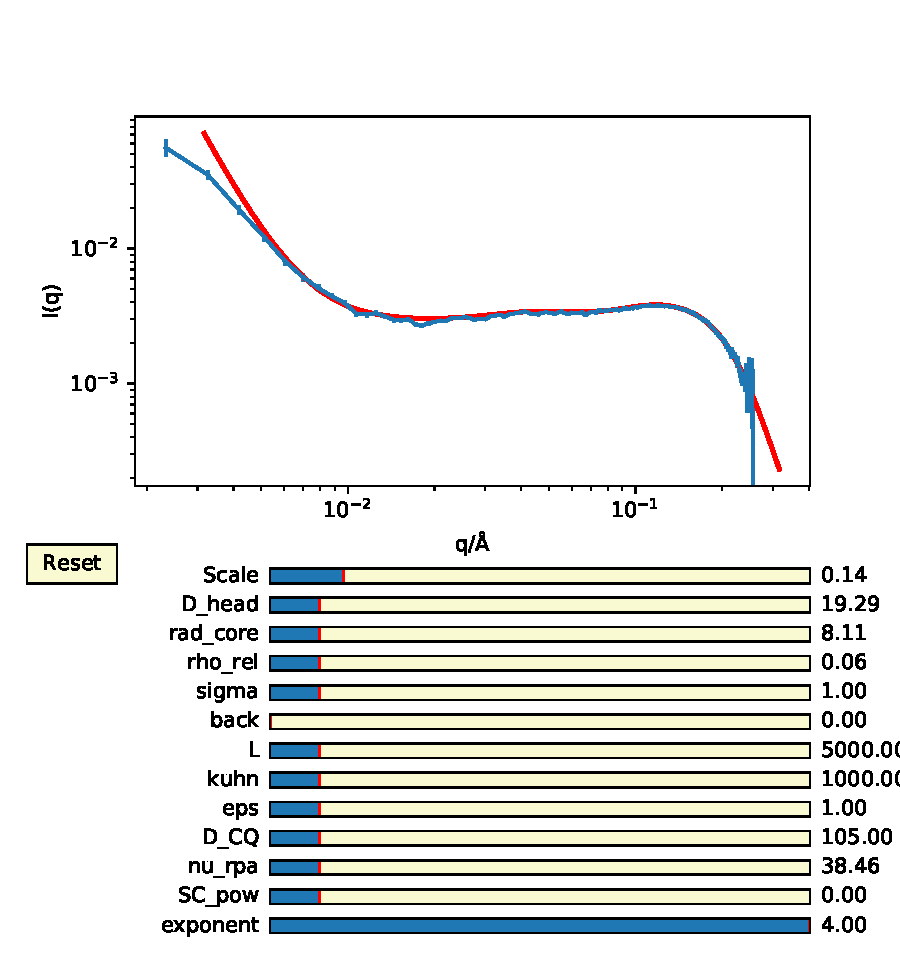
\includegraphics[width=0.7\textwidth]{imagens/saxs/Modelo_dado_SAXS_python}
	\caption{Dado real (azul) e modelo (vermelho) junto com os parâmetros de ajuste utilizados no modelo}
	\label{fig:saxs_modelo_dado_saxs_python}
\end{figure}

	Uma das motivações para realizar essa tarefa foi a grande dificuldade de nosso grupo utilizar SAXS para estudar micelas. Não há especialistas na região que conhecem modelagem de micelas gigantes. Além disso, escrever um modelo computacional baseando-se somente as equações matemáticas é uma tarefa muito difícil para quem não possui experiência. O modelo computacional, apesar de menos compacto em sua notação, é mais fácil de ser utilizado pois os passos são bastante detalhados, o que também facilita o entendimento de novos alunos. Além disso, examinando o código, é possível notar vários detalhes operacionais, como constantes de integração/normalização que não estão explicitamente presentes nas equações.
	
	As equações descritas no apêndice anterior foram traduzidas em uma série de funções e termos dentro dessas funções. Para ajudar no entendimento, há comentários no código que referenciam as equações à medida que elas são utilizadas. Note, porém, que a lógica utilizada para descrever um modelo matematicamente e computacionalmente são diferentes. Matematicamente, iniciei descrevendo o modelo de forma geral e depois descrevi as partes mais detalhadas, enquanto que, computacionalmente, essa ordem pode se inverter.
	
	Para facilitar o entendimento, a tabela \ref{tab:AP_corrs_blocos_equacoes} correlaciona as equações e os blocos de código onde aparecem.

\begin{table}[H]
	\IBGEtab{%
		\caption{Blocos de código e equações}
		\label{tab:AP_corrs_blocos_equacoes}
	}%
	{%
	\begin{tabular}{c c}
		\toprule
		          Bloco           & Equações                                                                                                       \\ \midrule
		   \ref{lst:WLM_geral}    & \ref{eqn:AP_Fcs}, \ref{eqn:AP_Fwc}, \ref{eqn:AP_Rc}, \ref{eqn:AP_Rs}, \ref{eqn:AP_saxs_MG_geral}, \ref{eqn:AP_Fsphere}  \\
		  \ref{lst:cadeia_KP_1}   & Tab. \ref{tab_ap:AiBi}                                                                                                  \\
		  \ref{lst:cadeia_KP_2}   & \ref{eqn:AP_Si}, \ref{eqn:AP_xi}, \ref{eqn:AP_Fwc}, \ref{eqn:AP_chi}                                                  \\
		  \ref{lst:cadeia_KP_3}   & \ref{eqn:AP_Ai}, \ref{eqn:AP_Bi}, \ref{eqn:AP_Gamma}, \ref{eqn:AP_Fwc}                                                \\
		\ref{lst:cadeia_KP_Debye} & \ref{eqn:AP_fdebye}, \ref{eqn:AP_w}, \ref{eqn:AP_FchainExV}                                                          \\
		 \ref{lst:cadeia_KP_SI}   & \ref{eqn:AP_Si}                                                                                                    \\ \bottomrule
	\end{tabular}%
}{}
\end{table}

As seguintes equações não aparecem no código:

\begin{table}[H]
	\IBGEtab{%
		\caption{Equações não descritas}
		\label{tab:AP_equacoes_n_descritas}
	}%
	{%
		\begin{tabular}{c p{10cm}}
			\toprule
			Equação   & Motivo  \\ \midrule
			\ref{eqn:AP_saxs_MG_superficial} & Melhor descrita pela Eq. \ref{eqn:AP_saxs_MG_geral} \\
			\ref{eqn:AP_saxs_PRISM} & O modelo PRISM, com uma aproximação, é calculado dentro da Eq. \ref{eqn:AP_saxs_MG_geral}  \\
			\ref{eqn:AP_Fwc_dois_casos} & Os dois casos são considerados simulaneamente durante os cálculos, então não é preciso realizar uma divisão explícita no código dos fatores \\
			\ref{eqn:AP_Rg2} & Devido aos parâmetros iniciais, o modelo não necessita calcular o raio de giro. \\
			\ref{eqn:AP_Frod}  & O modelo utiliza uma função para esfera ao invés de bastão no denominador, como uma aproximação \\ \bottomrule
		\end{tabular}%
	}{}
\end{table}

	\subsection{Código}

	\begin{listing}[H]
		\inputminted{python}{./python/cadeias_WLM_1.py}
		\caption{Cálculo das equações \ref{eqn:AP_saxs_MG_geral} e \ref{eqn:AP_Fsphere}}
		\label{lst:WLM_geral}
	\end{listing}
	
	\begin{listing}[H]
	\inputminted{python}{./python/cadeias_WLM_2.py}
	\caption{Aplicação da equação \ref{eqn:AP_saxs_MG_geral} para uma faixa de \q. É esta a função que deve ser importada em outros pacotes para fazer uso da modelagem}
	\label{lst:WLM_whole_q}
	\end{listing}
	
%	A parte mais complexa do modelo é justamente o modelo de Kratky-Porod com volume excluído para cadeias core-shell, e por isso merece uma subseção própria.

%	\subsection{Fator $F_{KPchain_{ExV}}$}
%	\label{sec:apendice_F_KPchain}
%	As equações da seção \ref{sec:equacoes_Fwc} relevantes ao cálculo do fator de cadeias com volume excluído então descritas nos códigos a seguir (listas \ref{lst:cadeia_KP_1}, \ref{lst:cadeia_KP_2}, \ref{lst:cadeia_KP_3}, \ref{lst:cadeia_KP_Debye}, \ref{lst:cadeia_KP_SI}).
%	
	\begin{listing}[H]
		\inputminted{python}{./python/cadeia_kratky_porod_inicial_1.py}
		\caption{Cálculo do fator de cadeias de Kratky-Porod com volume excluído (Parte 1/3)}
		\label{lst:cadeia_KP_1}
	\end{listing}

	\begin{listing}[H]
		\inputminted{python}{./python/cadeia_kratky_porod_inicial_2.py}
		\caption{Cálculo do fator de cadeias de Kratky-Porod com volume excluído (Parte 2/3)}
		\label{lst:cadeia_KP_2}
	\end{listing}

	\begin{listing}[H]
		\inputminted{python}{./python/cadeia_kratky_porod_inicial_3.py}
		\caption{Cálculo do fator de cadeias de Kratky-Porod com volume excluído (Parte 3/3)}
		\label{lst:cadeia_KP_3}
	\end{listing}

	\begin{listing}[H]
		\inputminted{python}{./python/cadeia_kratky_porod_inicial_4.py}
		\caption{Cálculo do fator de Debye}
		\label{lst:cadeia_KP_Debye}
	\end{listing}

	\begin{listing}[H]
		\inputminted{python}{./python/cadeia_kratky_porod_inicial_5.py}
		\caption{Cálculo numérico da integral cardinal}  % todo: encontrar um nome melhor
		\label{lst:cadeia_KP_SI}
	\end{listing}

\subsection{Uso do código}

Agora que todas as equações necessárias para descrever as micelas gigantes estão corretamente descritas programaticamente, é possível utilizar o modelo facilmente em outros projetos. Supondo que todas as funções criadas estejam num pacote chamado \texttt{SAXS\_FF}, é possível chamar a função e plotar um gráfico igual ao da Fig. \ref{fig:saxs_modelo_dado_saxs_python} com o seguinte código (\ref{lst:utilizando_modelo_WLM}), bastante simples:

\begin{listing}[H]
 	\inputminted{python}{./python/uso_modelo.py}
 	\caption{Exemplo de como utilizar o código de micelas gigantes para realizar um plot}  % todo: encontrar um nome melhor
 	\label{lst:utilizando_modelo_WLM}
\end{listing}
	
A partir deste ponto, é possível utilizar o código para realizar plotagens interativas, como também ajustes, utilizando métodos como \texttt{curve\_fit} do \texttt{scipy.optimize} ou, idealmente, o pacote \texttt{lmfit}.

\section{Descrição e uso do software de tratamento de curvas de fluxo}

Para o tratamento de dados de curva de fluxo, foi criado um programa que permite o usuário aplicar três modelos mais complexos e um modelo simplificado para a obtenção de valores de viscosidade no repouso. Todas as amostras, sem exceção, demonstraram ser pseudoplásticas, então não foram colocados mais modelos. A seguir, será mostrado os modelos utilizados e seções da lógica do programa, pois o código fonte inteiro é longo demais (aproximadamente 1000 linhas).

\subsection{Modelos de curvas de fluxo pseudoplásticas}
\label{sec:modelagem_curva_fluxo}
Foram implementados os modelos de \emph{Carreau-Yasuda} (Eq \ref{eqn:AP_CarreauYasuda}), \emph{Carreau} (Eq. \ref{eqn:AP_Carreau}), \emph{Cross} (Eq. \ref{eqn:AP_Cross}) e \emph{linear}, de maior para menor complexidade, respectivamente. Os modelos correlacionam a taxa de cisalhamento ($\dot{\gamma}$, variável independente) à viscosidade ($\eta$, variável dependente) utilizando alguns parâmetros.

\begin{equation}
	\eta = \eta_{\infty} + \frac{\eta_0 - \eta_{\infty}}{\left[  1 + \left(  \dfrac{\dot{\gamma}}{\dot{\gamma}_b}  \right)^{a}  \right]^{\frac{ \left(  n - 1  \right) }{a}}}
	\label{eqn:AP_CarreauYasuda}
\end{equation}

\begin{equation}
	\eta = \eta_{\infty} + \frac{\eta_0 - \eta_{\infty}}{\left[  1 + \left(  \dfrac{\dot{\gamma}}{\dot{\gamma}_b}  \right)^{2}  \right]^{\frac{n}{2}}}
	\label{eqn:AP_Carreau}
\end{equation}

\begin{equation}
	\eta = \eta_{\infty} + \frac{\eta_0 - \eta_{\infty}}{1 + \left(  \dfrac{\dot{\gamma}}{\dot{\gamma}_b}  \right)^{n}}
	\label{eqn:AP_Cross}
\end{equation}

O modelo linear considera somente valores de viscosidade em $\dot{\gamma}$ próximos de zero, ou seja, $\eta = \eta_0 + 0 \times \dot{\gamma}$.

Os parâmetros possuem os seguintes significados:

\begin{table}[H]
	\IBGEtab{%
          \caption{Parâmetros dos modelos de fluidos pseudoplásticos}
		  \label{tab:params_pseudoplasticos}
		}%
		{%
		\begin{tabular}{c c p{9cm}}
			\toprule
			   Parâmetro     & Unidade   & Significado                                                     \\ \midrule
			    $\eta_0$     & Pa.s      & Viscosidade no repouso*                                         \\
			$\eta_{\infty}$  & Pa.s      & Viscosidade no infinito                                         \\
			      $n$        & --        & Inclinação da região de decaimento de viscosidade               \\
			$\dot{\gamma}_b$ & s\menosUm & $\dot{\gamma}$ de início da região de decaimento de viscosidade \\ \midrule
			      $a$        & --        & Afeta tanto a inclinação quanto o ponto de inflexão             \\ \bottomrule
		\end{tabular}%
		}{}
\end{table}
% todo: encontrar a unidade de GPb
% todo: pensar em colocar os gráficos mostrando como esses parâmetros afetam as curvas
% todo: pensar um pouco mais sobre o Carreau-Yasuda e como que o a deve se comportar

A Fig. \ref{fig:reologia_modelos} exemplifica os modelos de Carreau e Cross e como os parâmetros afetam o formato das curvas. Note que a escala dos eixos é logarítmica. Vemos que, essencialmente, ambas as curvas possuem formatos muito semelhantes, com os parâmetros escolhidos. A escolha de um modelo depende da qualidade dos dados e do desejo do experimentalista. Observando-se como os modelos variam com os parâmetros, nota-se que a queda de viscosidade do modelo de Carreau é menos abrupta que no modelo de Cross e se assemelha mais aos dados estudados, então esse modelo foi mais utilizado.

\begin{figure}[H]
	\begin{subfigure}[t]{0.45\textwidth}
		\centering
		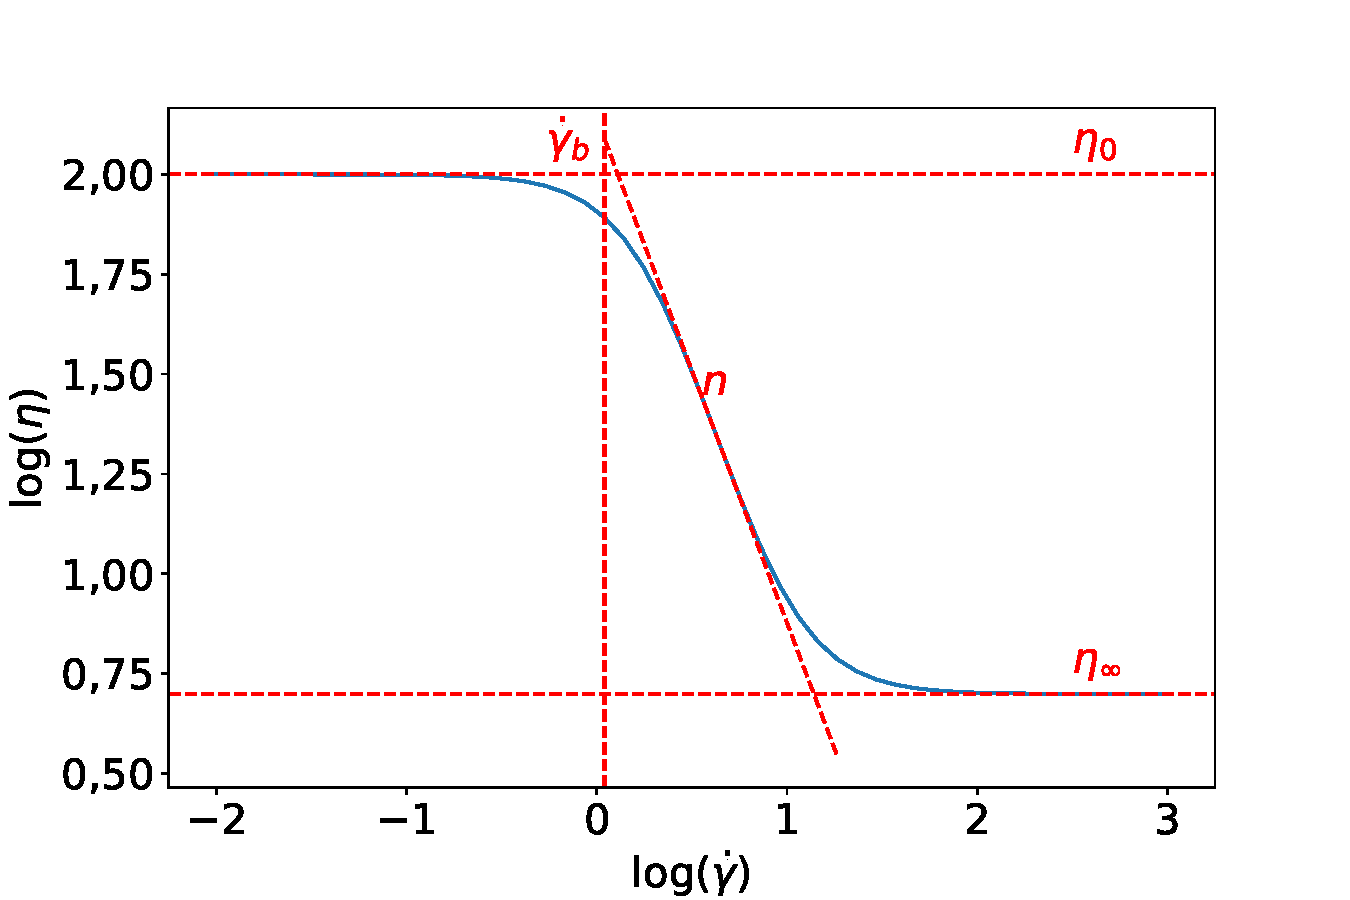
\includegraphics[width=\textwidth]{./imagens/reologia/Carreau}
		\caption{Modelo de Carreau}
		\label{fig:reologia_modelo_carreau}
	\end{subfigure} \qquad %
	\begin{subfigure}[t]{0.45\textwidth}
		\centering
		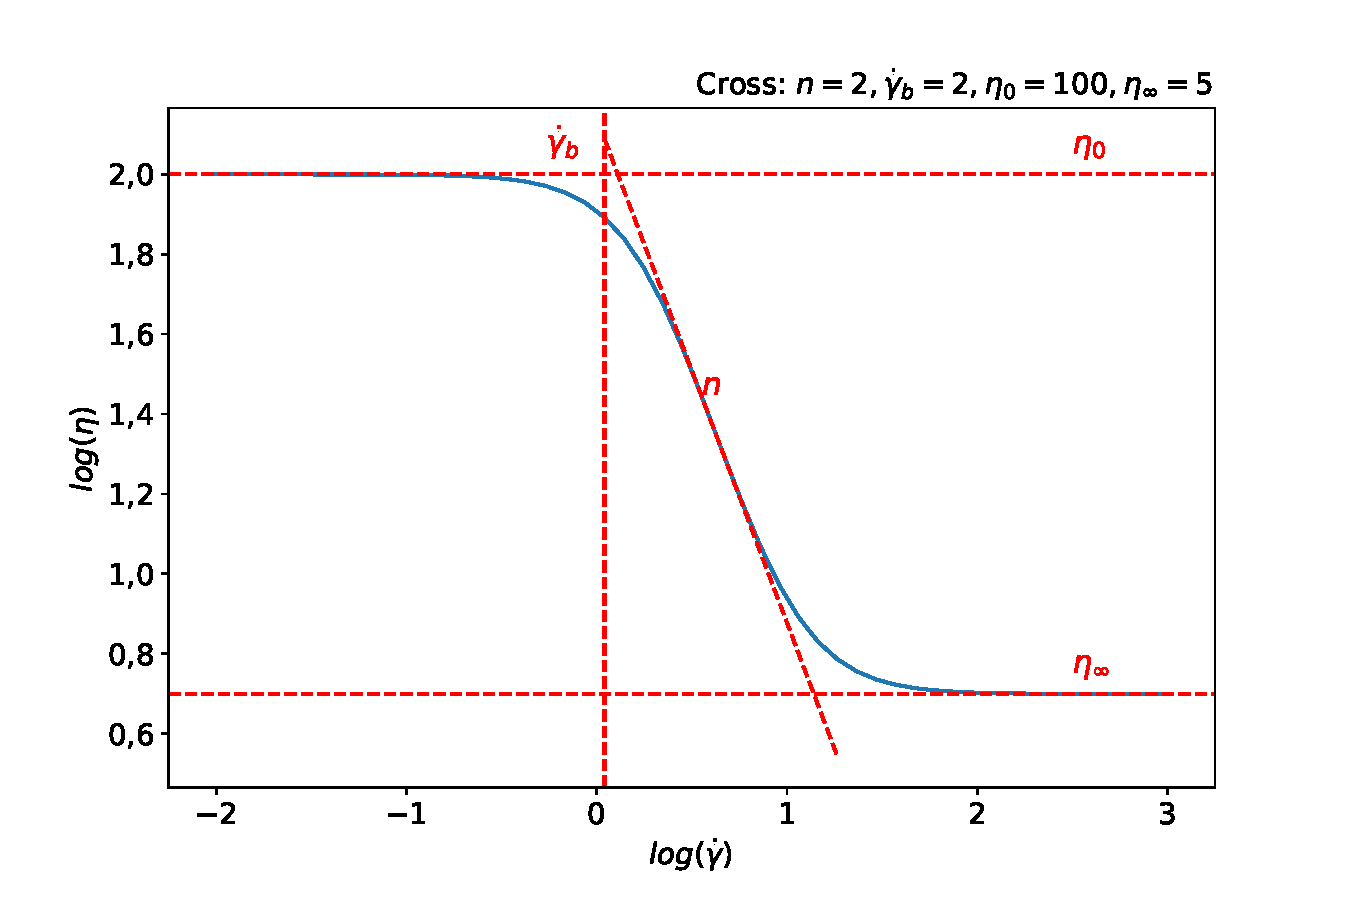
\includegraphics[width=\textwidth]{./imagens/reologia/Cross}
		\caption{Modelo de Cross}
		\label{fig:reologia_modelo_cross}
	\end{subfigure}
	\caption{Exemplos de curvas de fluxo descritas pelos modelos de Carreau e Cross, com os parâmetros utilizados.}
	\label{fig:reologia_modelos}
\end{figure}

De maior interesse para os estudos neste trabalho é a viscosidade no repouso, $\eta_0$, e portanto esse é o foco do programa. Porém, o ajuste indiscriminado de um modelo a um dado experimental é problemático caso a qualidade do dado não seja boa, seja pela própria característica da amostra, ou pela sensibilidade do equipamento. Por exemplo, é frequente que apareçam artefatos de medida em baixos valores de $\dot{\gamma}$, resultando ou num decréscimo ou acréscimo gradual de $\eta$. Além disso, é possível que não seja observada a região descrita por $\eta_{\infty}$, em altos valores de $\dot{\gamma}$, o que atribui grande incerteza na determinação desse parâmetro. Dessa forma, é necessário que uma região das curvas seja escolhida para que o ajuste seja bem sucedido e informativo, o que representa a maior dificuldade nesse tipo de análise, devido à certa subjetividade no critério de escolha da região de ajuste.

Por essa razão, e outras, como velocidade de análise, foi escrito o método de ajuste. O método consiste em realizar ajustes sucessivos, entre um ponto inicial $P_i$ até um ponto final $P_f$, e depois comparar os resultados dos ajustes para escolher um deles. Podem ser comparados, por exemplo, os parâmetros $R^2$, $\chi^2$ ou $\chi_{red}^2$. Escolhido o melhor ajuste, observando-se, por exemplo, a maior proximidade de $R^2$ a 1 ou de $\chi^2$ a 0, tomando cuidado para não escolher uma faixa muito estreita de pontos, os resultados são graficados, gravados num arquivo de texto e passa-se para o próximo dado experimental.

A listagem \ref{lst:exemplo_curva_de_fluxo} mostra duas seções do código completo do programa, uma mostrando o ciclo de ajuste utilizando o ajuste linear e \texttt{curve\_fit} e outro que realiza um ajuste não-linear utilizando o modelo de Carreau e \emph{lmfit}.

\begin{listing}[H]
	\inputminted{python}{./python/curva_de_fluxo.py}
	\caption{Seções do código mostrando o método de ajuste}  % todo: encontrar um nome melhor
	\label{lst:exemplo_curva_de_fluxo}
\end{listing}

Essas funções estão dentro de uma classe chamada \texttt{Fitter}. Para utilizar essa classe em outros códigos, é necessário inicializar uma instância da classe \texttt{Settings} e depois inicializar uma instância da classe \texttt{Fitter} utilizando as configurações da classe \texttt{Settings}. Caso não haja um arquivo \texttt{settings.dat} na pasta, um arquivo com valores padrão será criado. Após isso, é possível tanto editar o arquivo \texttt{settings.dat} quando utilizar as funções \texttt{print\_settings, edit\_settings} do objeto \texttt{Settings}. Ao criar um objeto \emph{Fitter}, por padrão os ajustes configurados já são realizados e os resultados são mostrados na tela. Caso se deseja criar um gráfico mostrando o resultado dos ajustes, pode-se chamar a função \texttt{plot\_error\_graphs()}. 

A listagem \ref{lst:exemplo_fitter} mostra como o programa pode ser utilizado por outros scripts, e o resultado do ajuste se encontra na Fig. \ref{fig:reologia_dado-exemplo}

\begin{listing}[H]
	\inputminted{python}{./python/uso_fitter.py}
	\caption{Exemplo de como utilizar a ferramenta de ajuste não linear}  % todo: encontrar um nome melhor
	\label{lst:exemplo_fitter}
\end{listing}

\begin{figure}[H]
	\centering
	\includegraphics[width=\textwidth]{imagens/reologia/Dado-exemplo}
	\caption{Figura resultante do ajuste não linear de Carreau e ajuste linear gerada pela função \texttt{plot\_error\_graphs()}. As barras de erro são oriundas da propagação de erro dos parâmetros e os números em vermelho indicam os pontos iniciais e finais considerados em cada ajuste.}
	\label{fig:reologia_dado-exemplo}
\end{figure}

Note que no dado utilizado, não há muitos problemas de desvio da curva, então os ajustes foram bem comportados. Os exemplos das figuras \ref{fig:reologia_dado-problemadescida} e \ref{fig:reologia_dado-problemasubida} mostram problemas reais na região de baixos valores de $\dot{\gamma}$.

\begin{figure}
	\centering
	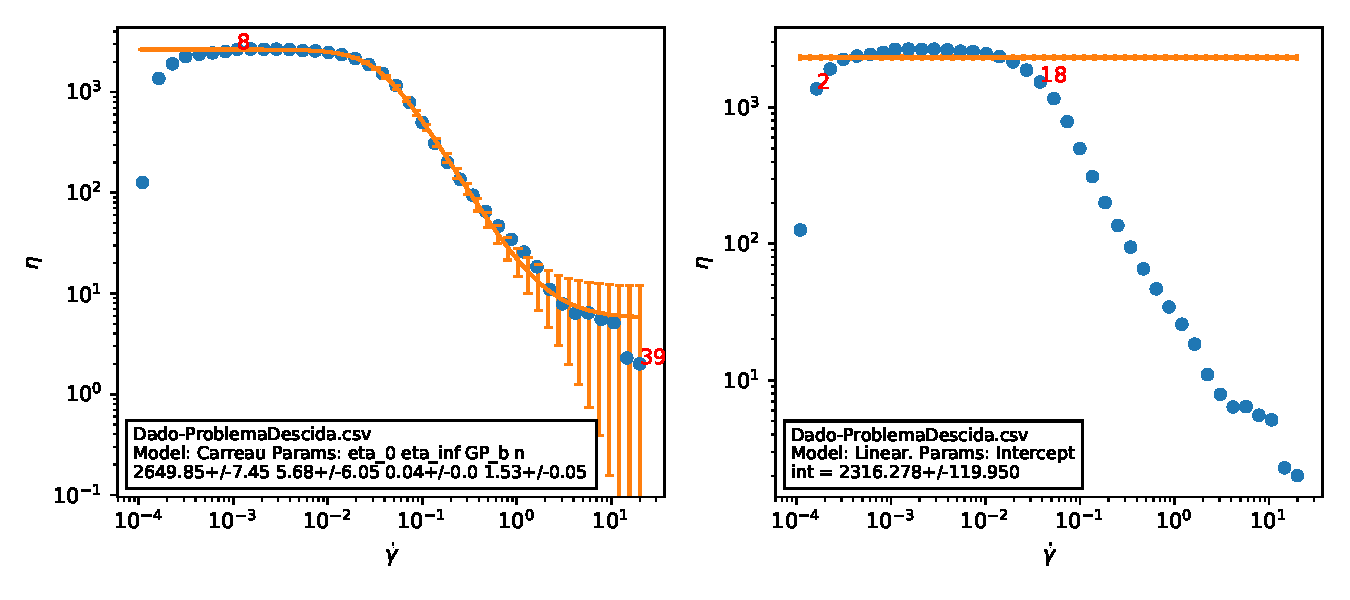
\includegraphics[width=\textwidth]{imagens/reologia/Dado-ProblemaDescida}
	\caption{Exemplo dos ajustes não-linear e linear de um dado real que possui uma queda nos valores de $\eta$ em baixas $\dot{\gamma}$}
	\label{fig:reologia_dado-problemadescida}
\end{figure}

\begin{figure}
	\centering
	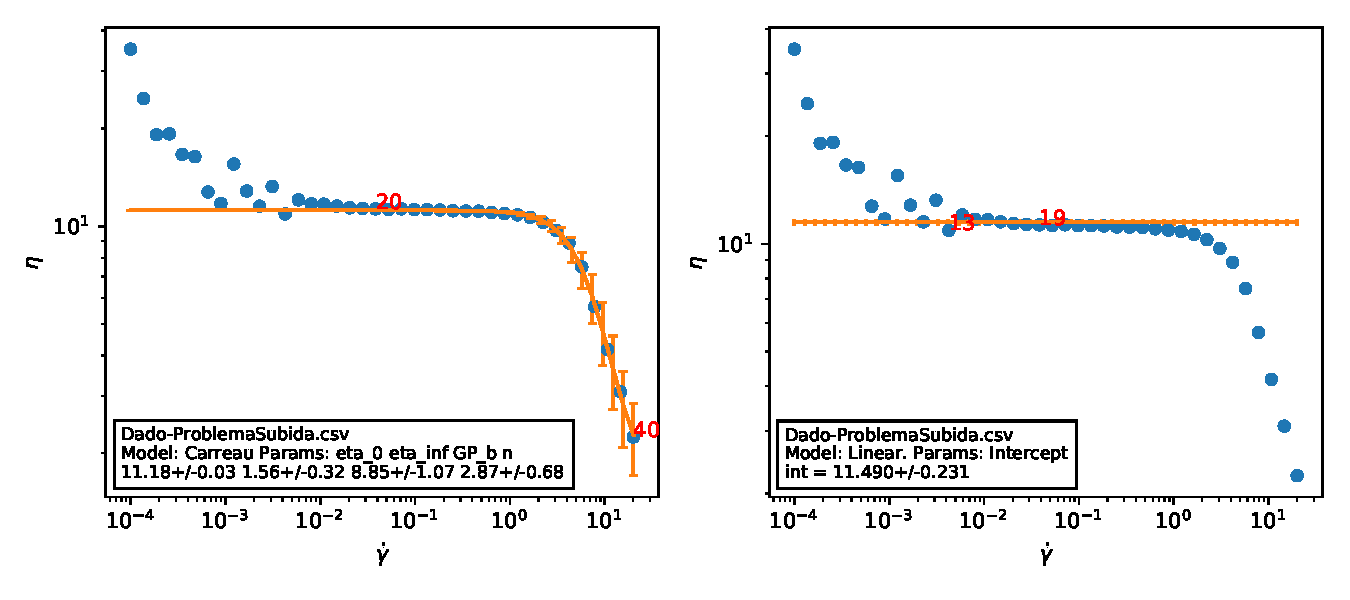
\includegraphics[width=\textwidth]{imagens/reologia/Dado-ProblemaSubida}
	\caption{Exemplo dos ajustes não-linear e linear de um dado real que possui um aumento nos valores de $\eta$ em baixas $\dot{\gamma}$}
	\label{fig:reologia_dado-problemasubida}
\end{figure}

O tempo de execução e de plotagem para cada experimento está na faixa de um segundo, o que é muito mais rápido do que realizar o ajuste manualmente em uma ferramenta como o Origin ou Excel, então é algo ideal para o tratamento de um grande volume de dados.

\section{Método de ajuste para reologia oscilatória de muco}

Durante a execução do projeto de doutorado, foi estabelecida uma parceria com uma aluna de doutorado da Faculdade de Ciências Médicas na Unicamp, Carla Cristina S. Gomez, para a análise de amostras de muco de pacientes com fibrose cística. Foram realizadas medidas de curva de fluxo, analisadas pelo método descrito na seção \ref{sec:modelagem_curva_fluxo}. Além disso, foi necessário realizar uma análise das curvas de varredura de frequência para obter informações relevantes.

Plotando-se todos os dados obtidos, observou-se que G' estava sempre acima de G'' e, na escala logarítmica, as duas curvas eram praticamente paralelas e ligeiramente inclinadas positivamente. Em alguns casos, a inclinação aumentava em frequências maiores e, frequentemente, havia uma oscilação de G' e G'' sem significado físico nessa região. A taxa de aumento era consistente com uma exponencial. Visto isso, foi desenvolvido um script que realiza o seguinte:

\begin{enumerate}
	\item Obter a região de frequência confiável de G' e de G'' para o modelo linear e exponencial. Isso é feito realizando-se ajustes gradativos, do primeiro ponto até um ponto \emph{n}, armazenando os ajustes e depois escolhendo o ajuste com maior número de pontos onde $R^2 > 0,9$. Caso não exista ajuste seguindo esse critério, escolhe-se um novo critério com $R^2 > 0,85$. Caso não exista ajuste que obedeça isso mesmo assim, é escolhido o ajuste com o maior número de pontos. 
	\item Os parâmetros dos ajustes que passaram pelo filtro de $R^2$ são gravados em um arquivo \texttt{csv}. Além disso, são gravados a média dos valores de G' e G'' da região linear, o desvio dessa média, o valor de $R^2$, os índices dos pontos utilizados para o ajuste e o valor de G' e G'' em 0,6813Hz. Esses parâmetros foram escolhidos com base em alguns artigos da literatura. % todo: ref?
\end{enumerate}

Cerca de 500 dados experimentais únicos são tratados e plotados em cerca de 3 minutos, mostrando novamente o ganho enorme de eficiência com métodos computacionais. Após análise estatística, observou-se uma variação significativa em um dos conjuntos de dados. Porém devido à enorme variabilidade das amostras, houve pouca relevância estatística no resto do conjunto de dados. Contudo, os pacientes revelaram uma melhora física após o tratamento estabelecido, mostrando que de fato o tratamento foi eficiente. Mais informações sobre esse projeto podem ser encontrados na tese da aluna. % todo: colocar uma referência pra tese dela.

\section{Softwares miscelâneos para tratamento de dados}


\end{apendicesenv}

%\begin{anexosenv}
%
%% Imprime uma página indicando o início dos anexos
%\partanexos
%
%% ---
%\chapter{Morbi ultrices rutrum lorem.}
%% ---
%\lipsum[30]
%
%% ---
%\chapter{Cras non urna sed feugiat cum sociis natoque penatibus et magnis dis
%parturient montes nascetur ridiculus mus}
%% ---
%
%\lipsum[31]
%
%% ---
%\chapter{Fusce facilisis lacinia dui}
%% ---
%
%\lipsum[32]
%
%\end{anexosenv}
